\documentclass[8pt, xcolor={svgnames}, hyperref={linkcolor=black}]{beamer}
\usepackage[labelfont={color=amethyst,bf}]{caption}
\setbeamercolor{background canvas}{bg=white}
\usetheme[progressbar=frametitle]{metropolis}
\usepackage{appendixnumberbeamer}
\usepackage{url}
\usepackage{booktabs}
\usepackage{braket}
\usepackage[scale=2]{ccicons}
\usepackage{amsfonts} 
\usepackage{amssymb}
\usepackage[english]{babel}
\colorlet{col1}{teal}
\colorlet{col2}{yellow}
\colorlet{col3}{green}
\usepackage{fontawesome}
\usepackage{subcaption}
\usepackage{multicol}
\usepackage{bm}
\usepackage{algorithm}
\usepackage{algpseudocode}
\usepackage{enumitem}

\usepackage[]{pseudo}


\usepackage{tikz}
\usetikzlibrary{positioning,arrows,calc,math,angles,quotes}
\usepackage{blochsphere}

\usetikzlibrary{arrows,automata}
\usetikzlibrary{positioning}
\usetikzlibrary{arrows.meta,
                bending,
                intersections,
                quotes,
                shapes.geometric}

\tikzset{
    state/.style={
           rectangle,
           rounded corners,
           draw=black, very thick,
           minimum height=1em,
           inner sep=2pt,
           text centered,
           },
}


\definecolor{myv}{rgb}{0.36, 0.22, 0.33}
\definecolor{gio}{rgb}{0.45, 0.31, 0.59}
\definecolor{light}{rgb}{0.8, 0.8, 1}
\definecolor{warmblack}{rgb}{0.0, 0.26, 0.26}
\definecolor{brown(web)}{rgb}{0.65, 0.16, 0.16}
\definecolor{cadmiumgreen}{rgb}{0.0, 0.42, 0.24}
\definecolor{darkmidnightblue}{rgb}{0.0, 0.2, 0.4}
\definecolor{brightube}{rgb}{0.82, 0.62, 0.91}

\definecolor{codegreen}{rgb}{0,0.6,0}
\definecolor{codegray}{rgb}{0.5,0.5,0.5}
\definecolor{codepurple}{rgb}{0.58,0,0.82}
\definecolor{backcolour}{rgb}{0.95,0.95,0.92}
\definecolor{amethyst}{rgb}{0.6, 0.33, 0.73}

\definecolor{light-gray}{gray}{0.95}
\newcommand{\code}[1]{\colorbox{light-gray}{\texttt{#1}}}

\usepackage[most]{tcolorbox}
\usepackage{xcolor}

%\usepackage[citecolor = green, linkcolor = blue, bookmarks=true, urlcolor=blue,
%colorlinks=true, pagebackref=true]{hyperref}


%\usepackage{xspace}

\title{Real-time quantum error mitigation in training VQAs}
\date{}
\author[Matteo Robbiati, Alejandro Sopena, Andrea Papaluca, Stefano Carrazza]{Matteo Robbiati, Alejandro Sopena, Andrea Papaluca, Stefano Carrazz}
\titlegraphic{
\begin{tikzpicture}[overlay, remember picture]

\node[at=(current page.south east), anchor=south east] {%

\includegraphics[width=.18\textwidth]{figures/qibo.png} 

\includegraphics[width=.18\textwidth]{figures/unimi.png} 

\includegraphics[width=.18\textwidth]{figures/cern.png}  

\includegraphics[width=.18\textwidth]{figures/qti.png}  
};
\end{tikzpicture}
}



\begin{document}

\begin{frame}{RTQEM pipeline}
We define a Real-Time Quantum Error Mitigation (RTQEM) procedure.
\begin{figure}
    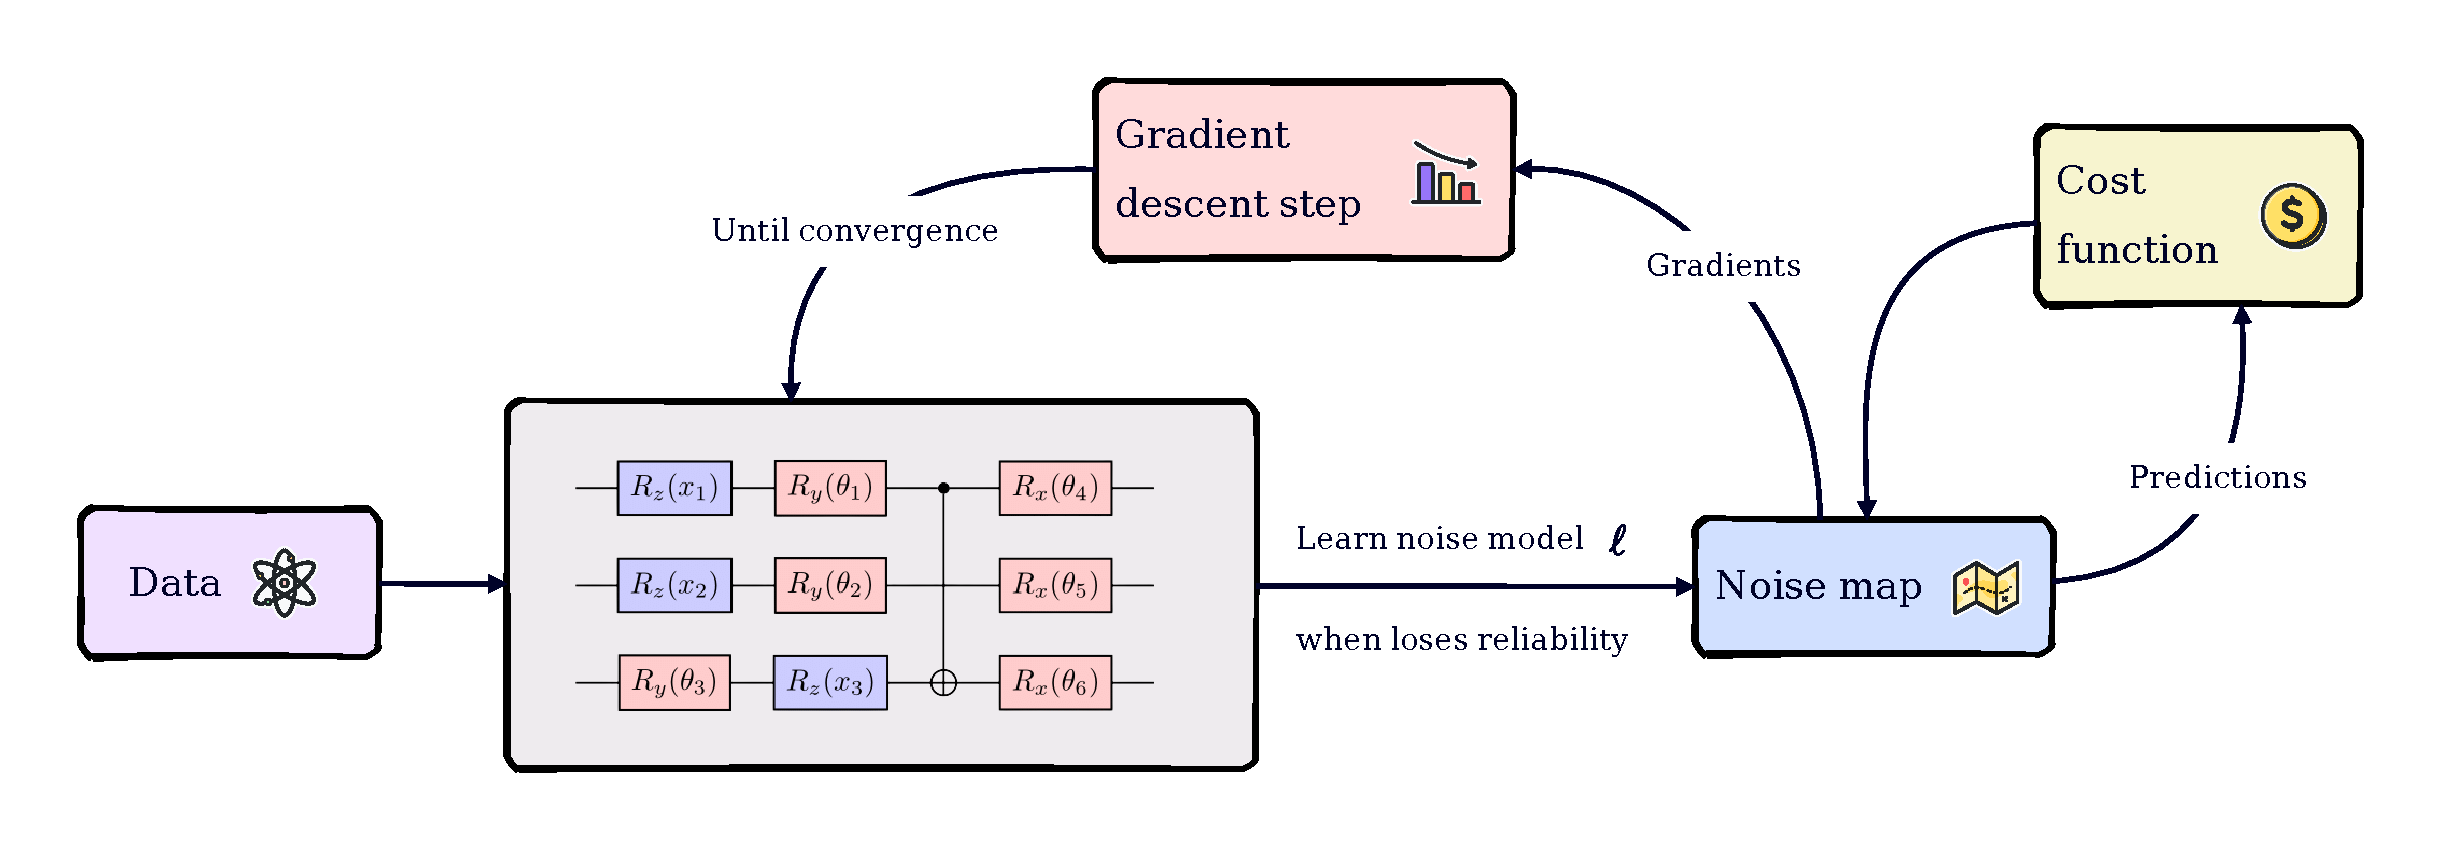
\includegraphics[width=1\textwidth]{figures/rtqem.pdf}
\end{figure}
\begin{itemize}[noitemsep]
\item[1.] consider a Variational Quantum Algorithm trained with gradient descent;
\item[2.] learn the noise map $\ell$ every time is needed over the procedure;
\item[3.] use $\ell$ to clean up both predictions and gradients.
\end{itemize}
\end{frame}

\begin{frame}{Learning the noise model \hfill \href{https://arxiv.org/abs/2112.06255}{\faBook\,\, arXiv:2112.06255}}
We use the Importance Clifford Sampling (ICS) procedure to learn the noise map $\ell$.
\begin{figure}
    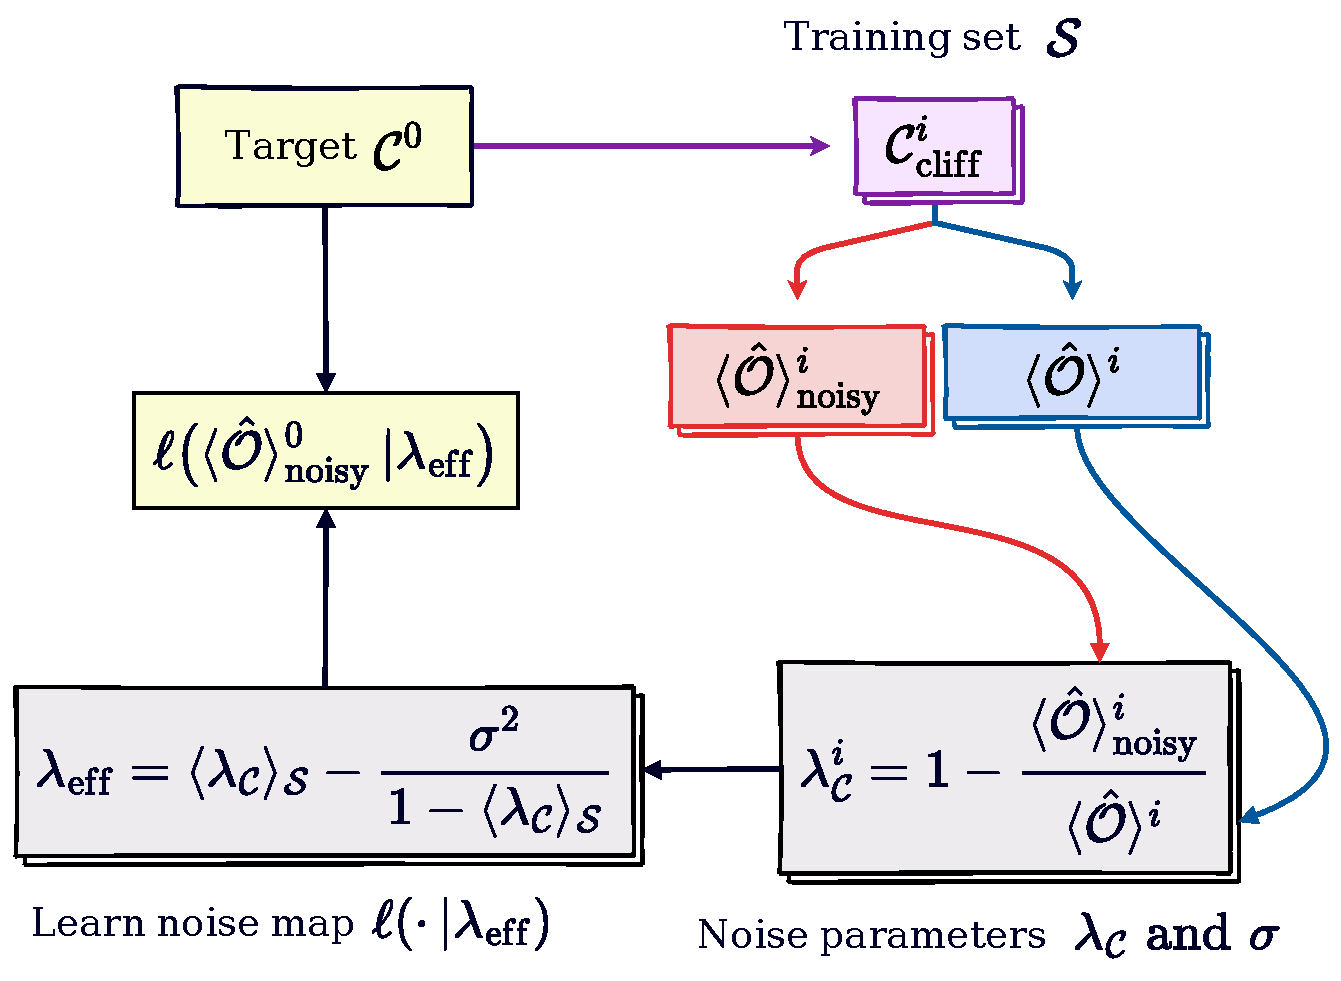
\includegraphics[width=0.65\textwidth]{figures/ics.pdf}
\end{figure}
\begin{itemize}[noitemsep]
\item[1.] sample a training set of Clifford circuits on top of a target $\mathcal{C}^0$;
\item[2.] process them so that their expectation values on Pauli strings is  $+1$ or $-1$;
\item[3.] QEM parameters $(a,  \sigma_a)$ are computed comparing exact values with noisy ones;
\item[4.] build $\ell$ following the Phenomenological-Error-Model Inspired (PEMI) protocol:
$$ \ell\bigl( \langle \hat{\mathcal{O}} \rangle | a, \sigma_a \bigr) = \frac{1-a}{[(1-a)^2 + 
\sigma_a^2]} \langle \hat{\mathcal{O}} \rangle_{\rm noisy} $$
\end{itemize}
\end{frame}

\begin{frame}{One dimensional HEP target: the $u$-quark PDF}

\begin{center}
\footnotesize
\begin{tabular}{ccccccccc}
\hline \hline 
\rule{0pt}{2.5ex}
\textbf{Parameter} & $N_{\rm train}$ & $N_{\rm params}$ & $N_{\rm shots}$ 
& $\text{MSE}_{\rm best}^{\rm rtqem}$ &  $\text{MSE}_{\rm best}^{\rm unmit}$ & Noise \\
\hline
\rule{0pt}{2.5ex}
\textbf{Value} & $30$ & $16$ & $10^{4}$ &  $1.1 \cdot 10^{-3}$ & $6.1 \cdot 10^{-3}$ & local Pauli \\
\hline \hline 
\end{tabular}
\end{center}

\begin{figure}
    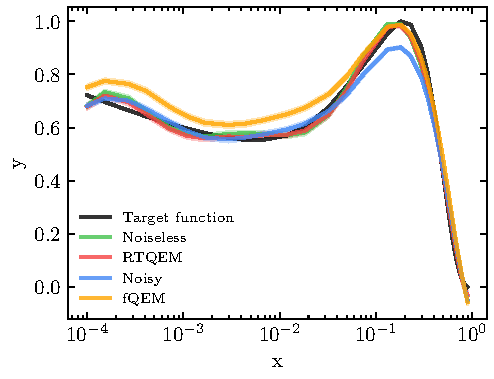
\includegraphics[width=0.5\textwidth]{figures/qpdf.pdf}%
    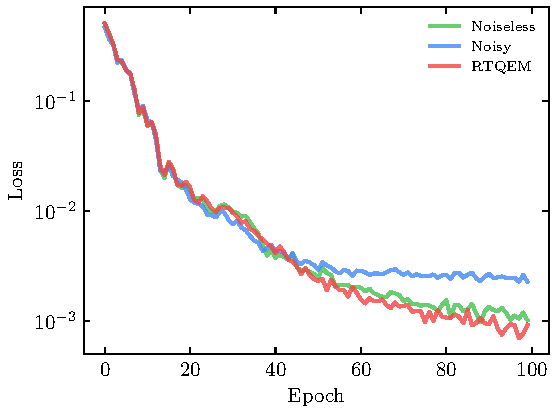
\includegraphics[width=0.5\textwidth]{figures/qpdf_loss.pdf}
\end{figure}
\begin{itemize}[noitemsep]
\item[1.] thanks to the RTQEM procedure, we reach a good minimum of the cost function;
\item[2.] the QEM is not effective is applied to a corrupted scenario (orange curve).
\end{itemize}
\end{frame}

\begin{frame}{Multidimensional target}
We tackle a multi-dimensional target computing predictions as expected value of 
a $Z^{\otimes N_{\rm \dim}}$ after executing an $N_{\rm \dim}$ circuit.

\begin{center}
\footnotesize
\begin{tabular}{ccccccccc}
\hline \hline 
\rule{0pt}{2.5ex}
\textbf{Job ID} & $N_{\rm train}$ & $N_{\rm params}$ & $N_{\rm shots}$ 
& $\text{MSE}_{\rm best}^{\rm rtqem}$ &  $\text{MSE}_{\rm best}^{\rm unmit}$ & Noise \\
\hline
$N_{\rm dim}=4$ & $30$ & $48$ & $10^{4}$ &  $4.4 \cdot 10^{-4}$ & $1.9 \cdot 10^{-2}$ & local Pauli \\
$N_{\rm dim}=6$ & $30$ & $72$ & $10^{4}$ &  $4.1 \cdot 10^{-4}$ & $3.8 \cdot 10^{-2}$ & local Pauli \\
$N_{\rm dim}=8$ & $30$ & $96$ & $10^{4}$ &  $5.6 \cdot 10^{-4}$ & $4.8 \cdot 10^{-2}$ & local Pauli \\
\hline \hline 
\end{tabular}
\end{center}

\begin{figure}
    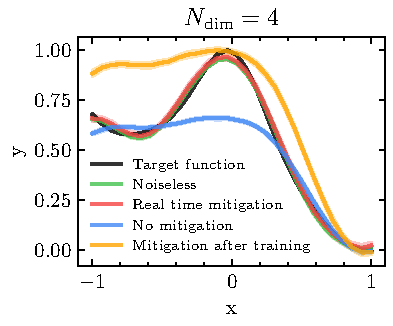
\includegraphics[width=0.31\textwidth]{figures/cos4d.pdf}%
    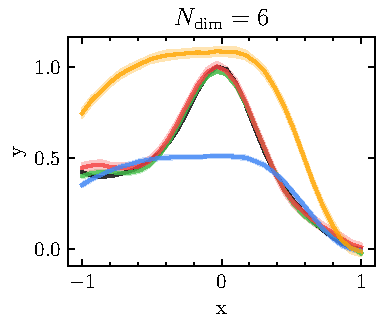
\includegraphics[width=0.31\textwidth]{figures/cos6d.pdf}%
    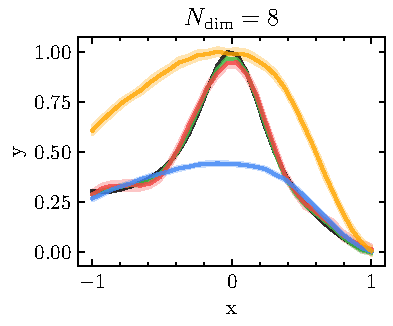
\includegraphics[width=0.31\textwidth]{figures/cos8d.pdf}
    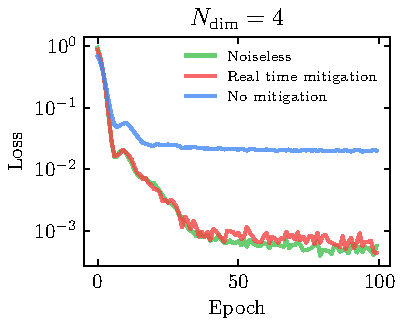
\includegraphics[width=0.31\textwidth]{figures/cos4d_loss.pdf}%
    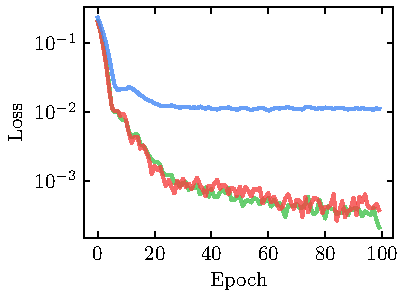
\includegraphics[width=0.31\textwidth]{figures/cos6d_loss.pdf}%
    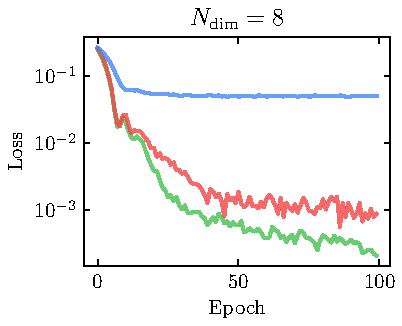
\includegraphics[width=0.31\textwidth]{figures/cos8d_loss.pdf}
\end{figure}
\end{frame}

\begin{frame}{RTQEM on a superconducting qubit}
% \begin{center}
% \footnotesize
% \begin{tabular}{ccccccccc}
% \hline \hline 
% \rule{0pt}{2.5ex}
% \textbf{Parameter} & $N_{\rm train}$ & $N_{\rm params}$ & $N_{\rm shots}$ 
% & $\text{MSE}_{\rm best}^{\rm rtqem}$ &  $\text{MSE}_{\rm best}^{\rm unmit}$ & Noise \\
% \hline
% \rule{0pt}{2.5ex}
% \textbf{Value} & $30$ & $16$ & $10^{4}$ &  $1.1 \cdot 10^{-3}$ & $6.1 \cdot 10^{-3}$ & local Pauli \\
% \hline \hline 
% \end{tabular}
% \end{center}

\begin{figure}
    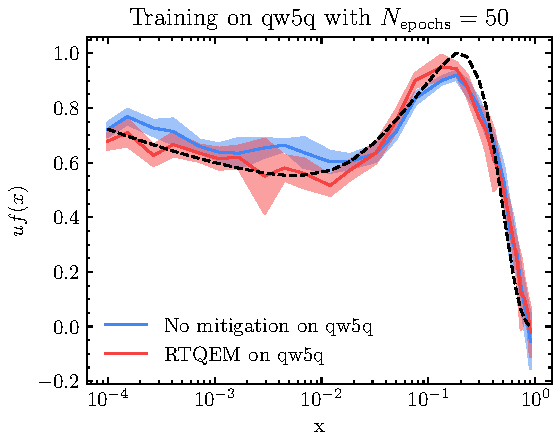
\includegraphics[width=0.5\textwidth]{figures/qw5q.pdf}%
    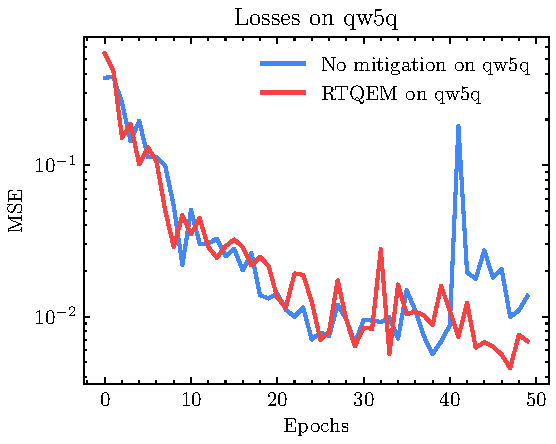
\includegraphics[width=0.5\textwidth]{figures/losses_qw5q.pdf}
\end{figure}
\end{frame}

\end{document}
